%%%%%%%%%%%%%%%%%%%%%%% file typeinst.tex %%%%%%%%%%%%%%%%%%%%%%%%%
%
% This is the LaTeX source for the instructions to authors using
% the LaTeX document class 'llncs.cls' for contributions to
% the Lecture Notes in Computer Sciences series.
% http://www.springer.com/lncs       Springer Heidelberg 2006/05/04
%
% It may be used as a template for your own input - copy it
% to a new file with a new name and use it as the basis
% for your article.
%
% NB: the document class 'llncs' has its own and detailed documentation, see
% ftp://ftp.springer.de/data/pubftp/pub/tex/latex/llncs/latex2e/llncsdoc.pdf
%
%%%%%%%%%%%%%%%%%%%%%%%%%%%%%%%%%%%%%%%%%%%%%%%%%%%%%%%%%%%%%%%%%%%


\documentclass[runningheads,a4paper]{llncs}

\usepackage{amssymb}
\setcounter{tocdepth}{3}
\usepackage{graphicx}
\usepackage{lscape}
\usepackage{url}
\usepackage{subfigure}
\urldef{\mailsa}\path|{wendpanga-francis.ouedraogo,frederique.biennier}@liris.cnrs.fr|
\urldef{\mailsb}\path|philippe.merle@inria.fr|    
\newcommand{\keywords}[1]{\par\addvspace\baselineskip
\noindent\keywordname\enspace\ignorespaces#1}

\begin{document}

\mainmatter  % start of an individual contribution

% first the title is needed
\title{Contextualised security operation deployment through MDS@run.time architecture}

% a short form should be given in case it is too long for the running head
\titlerunning{Contextualised security operation deployment through MDS@run.time}

% the name(s) of the author(s) follow(s) next
%
% NB: Chinese authors should write their first names(s) in front of
% their surnames. This ensures that the names appear correctly in
% the running heads and the author index.
%
\author{Wendpanga Francis Ouedraogo\inst{1}
\and Fr\'ed\'erique Biennier \inst{1} \and Philippe Merle\inst{2}}
% \authorrunning{Contextualised security deployment through MDS@run.time architecture}
% (feature abused for this document to repeat the title also on left hand pages)

% the affiliations are given next; don't give your e-mail address
% unless you accept that it will be published
\institute{Universit\'e de Lyon, CNRS INSA-Lyon, LIRIS UMR 5205, 20 avenue Albert Einstein, 69621 Villeurbanne Cedex, France\\
\mailsa\\
\and Inria Lille - Nord Europe, Parc Scientifique de la Haute Borne, 40 avenue Halley, 59650 Villeneuve d'Ascq, France\\
\mailsb\\}

%
% NB: a more complex sample for affiliations and the mapping to the
% corresponding authors can be found in the file "llncs.dem"
% (search for the string "\mainmatter" where a contribution starts).
% "llncs.dem" accompanies the document class "llncs.cls".
%

%\toctitle{Lecture Notes in Computer Science}
%\tocauthor{Authors' Instructions}

\maketitle

\begin{abstract}
The development of collaborative business leads to new challenges for corporate information systems such as interoperability, elastic deployment and security management in dynamic contexts. To fit these challenges one can take advantage of the agility and elasticity provided by Service Oriented Computing and Cloud Computing. To support an adaptive and contextualised security deployment providing a consistent protection level despite the changing contexts, we propose MDS@run.time that is the marriage of both Model Driven Security (MDS) and Models@run.time approaches. Security policy models (produced by a MDS process) are interpreted at runtime depending on the context (Models@run.time). To this end, we propose an architecture that can be plugged on any hosting middleware to manage the security mediation (i.e. select, compose and orchestrate security services) depending on the protection requirements defined in the security policies. A Security as a Service component is also proposed to support this "security outsourcing" strategy. This proposition is illustrated thanks to a Proof of Concept prototype built on top of the FraSCAti middleware.
\end{abstract}

\section{Introduction}
The development of collaborative business strategies leads to reorganize the corporate information system deployment in order to increase its agility. Taking advantage of the agility and interoperability of Service-Oriented Architecture (SOA), collaborative Business Process (BP) can efficiently be built by composing business services depending on business needs. Nevertheless, such collaborative organization challenges contextualized security deployment as a same business service may be used in different collaborative contexts and orchestrated using different runtime environments.
To fit this challenge, we have proposed to extend the Model Driven Security (MDS) approach~\cite{LS09} to capture information and service protection requirements using an “end-user oriented” set of questions to capture the patrimonial importance of these elements so that confidentiality, availability, and integrity requirements can be consistently defined and used to annotate the BP specification~\cite{OBG12}. Then we use a model-driven process to generate the security policies associated to the services implementing the collaborative BP.

In this paper, we propose MDS@run.time that is the marriage of both MDS and Models@run.time~\cite{blair2009models} approaches.
In brief, security policies produced by a MDS process are interpreted at runtime depending on the context.
Thus security policies are seen as an abstract Models@run.time protection specification.
Depending on the runtime environment, different security services must be selected and orchestrated to fulfill the protection requirements.
MDS@run.time is independent of any hosting middleware and
is plugged on them to manage the security mediation (i.e. select, compose and orchestrate security services) depending on the protection requirements defined in the security policies.
A MDS@run.time component intercepts each service invocation, extracts its security policy and orchestrates the required protection services depending on the execution environment before launching the “functional” service.
A Security as a Service component is also proposed to support this "security outsourcing" strategy. 
This approach is implemented by a proof of concept prototype built on top of the FraSCAti service-oriented middleware.


We first present the context and a motivating example (section ~\ref{contextAndMotivation})  before defining the way MDS is extended in a Security Models@run.time vision and the related architecture (section ~\ref{MDStoMDSatRuntime}). We detail the way this architecture is implemented and plugged on FraSCAti middleware (section ~\ref{mdsAtRuntimeWithFrascati}) and evaluate its performance (section ~\ref{sec:evaluation}) before confronting our proposal with the related works (section ~\ref{relatedwork}).

\section{Context and motivating example}
\label{contextAndMotivation}

The increased importance of collaborative business strategies leads to reorganize the corporate information system deployment in order to increase its agility and interoperability so that common BP supporting these collaborative organisations can be efficiently designed and deployed. Taking advantage of the agility and interoperability of SOA and Cloud environments, such collaborative BP can be built by composing business services before deploying them on cloud platforms depending on the needs. This leads to a "de-perimetrised" information system organisation, as business services can be selected, composed and orchestrated in various contexts, challenging a consistent and contextualised business service protection.

\subsection{Motivating example}
\label{example}

A motivating example illustrating a Collaborative Process organisation is presented Fig.~\ref{fig:bp}. Setting an e-government service to improve a scholarship management process leads to the development of a collaborative "on-line" e-governement organisation allowing both students, grant administration and academic partners to share students' curriculum information. To this end, a common BP associated to scholarship business feature is built, combining services and personal workflows from both grant administration and academic partners, challenging new security features such as partner authentication, access control, non repudiation on the student information. 


This collaborative BP is split among 3 lanes associated to the different participants (the student, the scholarship management service and the academic institution). Instead of exchanging paper/electronic forms containing student applications, curriculum information that must be the regional council opens its scholarship information system to allow academic institution and students to interact directly with the corresponding business services. As students' personal information are managed, a particular attention must be paid on privacy requirements. While any back-office scholarship employee can access without any control to the student scholarship resource, more precise authentication and authorisation processes must be deployed for the e-government execution: students can access via a secured connection to their own scholarship form whereas academic institution administrative staff should access to the validation forms for the students registered in one of their institution curriculum.

\begin{figure}
\centering
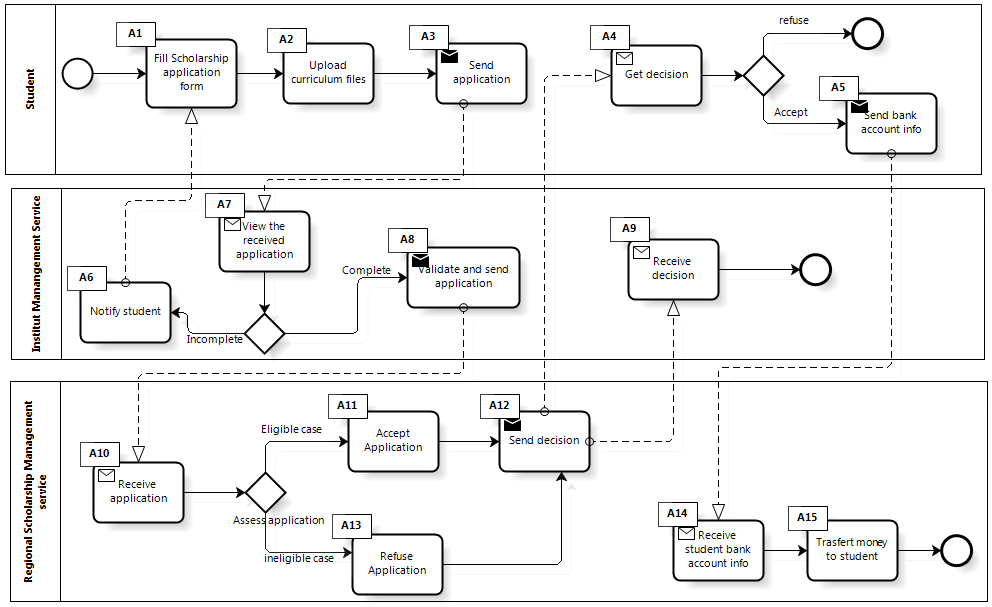
\includegraphics[height=220pt, width=\linewidth]{scholarshipBP.png}
\caption[Scholarship management process]{Scholarship management process.\\ The scholarship award collaborative process includes differents steps.Each student fills a scholarship application form, uploads various documents (resume, cover letter, diplomas, etc.) and submits its request. Then, the institute manager views and checks each student application data to ensure that it is compliant and sends it to the scholarship council. Applications are processed and decision are returned back before getting bank account information to process to the payment.}
\label{fig:bp}
\end{figure}
\subsection{Securing services}
Depending on the perceived security risks/system vulnerabilities, different security requirements can be set. Based on the ISO/IEC 27002, the OASIS Service Reference Model~\cite{OAS06} defines different security requirements (confidentiality and privacy management, integrity, authentication, authorisation, availability and non repudiation) that require the deployment of security means from the network layer, which is rather focused on the availability requirement and protection against deny of service attacks, and transport layer, which has to provide secured confidential channel between tranmitters and receivers, to the application layer, which manages most of the security requirements such as authentication, authorisation, non repudiation, confidentiality and privacy. Different standards such as WS-Security, SAML, XACML, BSLA, etc. have been developped to support and implement these security requirements.
Such protection means can either be deployed directly in the service operation or "attached" to the service interface specification. To this end, security policies can be used to specify the required protection levels and means to be deployed, allowing an easier "upgrading" of protection requirement. 



\begin{figure}  
\centering
\includegraphics[height=135pt, width=\linewidth]{scholarshipPolicies.png}
\caption{Security policies associated to the \textit{Scholarship}  resource.}
\label{fig:policy}
\end{figure}

Focusing on the service attached to the scholarship application form, a security policy can be set to define the different protection means to be deployed (see Fig.~\ref{fig:policy}). This service includes an operation named \textit{ViewStudentData}, which is considered as a resource (line 2 in
Fig.~\ref{fig:policy}). This resource requires authentication (lines 2-8) using a simple login/password process (line 4) refering to a checking file defined line 5. Besides authentication, access control (lines 9-16) using ACL (line 14), enforced with a time constraint (line 12) should be applied to this resource. Fig.~\ref{fig:acl} describes the contents of the authorization file defining that users can access to the resource only at a particular time period, e.g., between 6am and 12pm for \textit{user1}.
 
\begin{figure}
\centering
\includegraphics[height=55pt, width=\linewidth]{scholarshipAcl.png}
\caption{\textit{AccessControlList.xml} authorization file.}
\label{fig:acl}
\end{figure}



\section{From MDS to MDS@Run.time}
\label{MDStoMDSatRuntime}
Different methods can be used to set a consistent security policy based on vulnerability and threats models such as EBIOS, MEHARI, OCTAVE, SNA \footnote{https://www.enisa.europa.eu/activities/risk-management/current-risk/risk-management-inventory/rm-isms}. However, they are complex and designed for a perimetrised environment and are not end-user oriented. To overcome these limits, business architects should be able to define security policies while building new BP. To this end, MDS can be used to attach security requirements specification in the BP and generate adapted security policies.

\subsection{MDS for Services}
In previous work~\cite{OBG12}, we have proposed to enrich the MDS approach with a security pattern engineering strategy to capture protection requirements and deployment platform information to generate automatically the security policies that will be attached to the different services (see Fig.~\ref{fig:mds}).

\begin{figure}[ht!] 
\centering
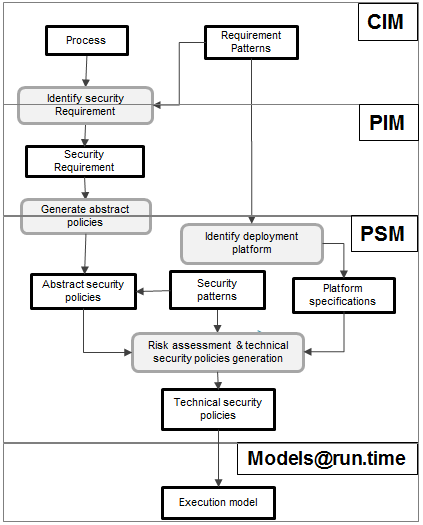
\includegraphics[height=220pt,width=200pt]{mds.png}
\caption{Security policy generation process based on MDS.}
\label{fig:mds}
\end{figure}

These security policies, which are in fact our security models at runtime, are associated with the service description (Fig.~\ref{fig:wsdl}, line 3). This allows during business service execution to identify the security policies to be applied.

\begin{figure}[ht!]  
\centering
\includegraphics[height=100pt, width=\linewidth]{scholarshipWSDL.png}
\caption{Link policy file with the \emph{ViewStudentData} operation of the \emph{Scholarship} service.}
\label{fig:wsdl}
\end{figure}

In our example, the student curriculum activity and the related information must be protected in the new \textit{opened} context. This confidentiality requirement impacts both application layer, which is in charge of the access control, i.e. authentication and authorisation management, and transport layer (see Fig.~\ref{fig:policy}). 

To provide a consistent protection of the information system, the security policies must be used to compose and orchestrate security services accordingly. Taking into account more precise information on the execution context could improve both the service operation performance and the protection level, avoiding under/over protection deployment. In our example, each employee of the academic partners can access to the curriculum activity from the already secured partner network. Once the security policy is attached to the collaborative workflow, access control including a systematic authentication is required to fulfill the non repudiation requirement as well as log features and network encryption, despite the secured access provided by the corporate infrastructure (namely authentication to unlock the workstation and secured infrastructure). Table~\ref{tab:tab1} shows a comparison of service execution time with/without authentication and authorization, testing conditions and environment are detailed in Section~\ref{sec:evaluation}.

\begin{table}
\caption{Service execution time.}
\begin{tabular}{|p{8cm}|c|}
\hline
Executed components & Execution time (ms)\\
  \hline
 Business service & 59\\
 Business service + Authentication & 69\\ 
 Business service + Authentication + Authorization & 72\\ 
    \hline
\end{tabular}
\label{tab:tab1}
\end{table}

To avoid this costly over protection or risky under protection depending on the runtime environment vulnerability, we propose to turn these security policies as Models@run.time so that they can be analysed to select, compose and orchestrate the most convenient security services depending on the exact runtime environment. This requires a new architecture to \textit{outsource} the security management as a new high-level service that can be plugged on the hosting middleware. In the next sections, we present this new architecture and a proof of concept based on the FraSCAti middleware.

\subsection{Adapting security deployment in service operation with MDS@run.time}

Implementing a Service Oriented Architecture (SOA) requires a middleware for both integration and distributed communication. Middleware plays an intermediary role between the client and the service provider. It is a software component, which is located between the operating system and business applications, and offers a high level abstraction for building distributed applications. It allows business service integration and management, and provides access to various external services~\cite{SHLP05}. It is an integration solution, which implements a fully distributed architecture deployed on multiple nodes, providing services such as data processing or Content Based Routing (CBR), and a higher level of interoperability by systematically using standards such as XML, Web Services specifications aka WS-*, ~\cite{FJF08}.
 
Our architecture is built on the traditional service/middleware/hosting platforms architecture (see Fig.~\ref{fig:archiA}). In order to avoid under or over protection depending on the runtime context, we propose to outsource the security management. As stated in the previous section, the security policy attached to each business service expresses the protection requirement for this service. Plugged on the classical business service/middleware/hosting cloud platform(s) architecture, our MDS@run.time architecture (see Fig.~\ref{fig:archiB}) consists in:

\begin{itemize}
\settowidth{\leftmargin}{{\Large$\square$}}\advance\leftmargin\labelsep
\itemsep5pt\relax
\renewcommand\labelitemi{{\lower1.5pt\hbox{\Large$\square$}}}
\item A middleware specific \texttt{Interceptor} component plugged on the middleware intercepts each service/middleware interaction (step 1) and routes this interaction to the \texttt{MDS@run.time} component (step 2).
\item	The \texttt{MDS@run.time} component is the core component to achieve the dynamic security deployment. It consists in three sub components:
\begin{itemize}
\item	The \texttt{policy manager} parses the service description, extracts and loads the associated policy files before launching the context acquisition process.
\item The \texttt{context manager} collects information associated to the execution context (steps 3 and 4). It transfers the results to the \texttt{security mediator}.
\item	The \texttt{security mediator} parses the security policy to get the protection level associated to each security service. Depending on the execution context, it selects and composes security services to implement the required protection. Then it orchestrates the security service invocations (steps 5 and 6) and if succeeded, it routes back the business service/middleware interaction to the middleware.
\end{itemize}
\item The \texttt{Security as a Service} component gathers implementation of various security services (authentication, authorisation, integrity controls, etc.).
\end{itemize}
\begin{figure}
    \centering
    \subfigure[Multi-layer architecture.]{\label{fig:archiA} 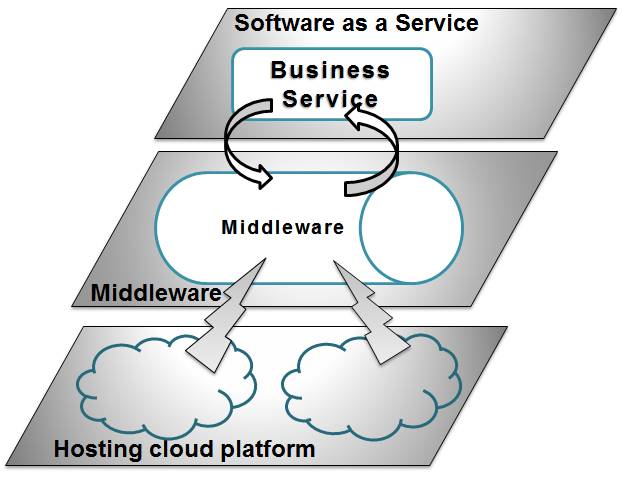
\includegraphics[height=120pt, width=120pt]{architecture2.PNG}}
    \subfigure[Multi-layer architecture with MDS@run.time.]{\label{fig:archiB} 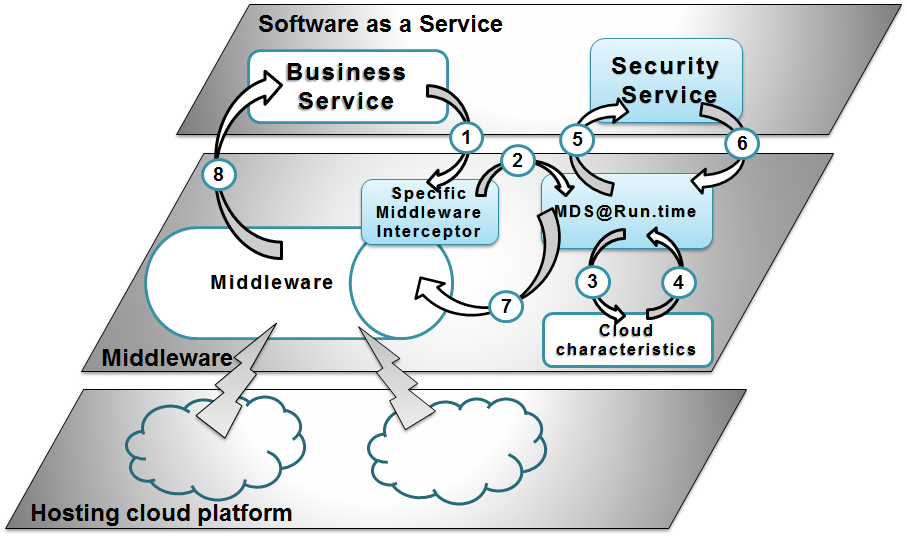
\includegraphics[height=180pt, width=215pt]{architecture1.PNG}}
    \caption{MDS@run.time architecture.}
    \label{fig:archi}
\end{figure}

\section{MDS@run.time with FraSCAti}
\label{mdsAtRuntimeWithFrascati}
FraSCAti\footnote{\url{http://frascati.ow2.org}}~\cite{SMF09} is an open source middleware framework to build, program, deploy, and execute adaptable service-oriented business applications.
FraSCAti is based on the OASIS Service Component Architecture (SCA) standard\footnote{\url{http://www.oasis-opencsa.org/sca}}. FraSCAti applications can be deployed in different clouds (Amazon EC2, Amazon Elastic BeanTalk, Google App Engine, CloudBees, etc.)~\cite{MRS11}\cite{PHM12}\cite{fawaz2013COMPJ}. The adaptability at design time is based on the fact that the FraSCAti platform was designed as a plugin-based architecture to adapt it to different execution environments and to select on demand the required application functionalities compose FraSCAti~\cite{acher:inria-00614984}. The adaptability at execution time is based on the FraSCAti reflective features, which encompass introspection and reconfiguration of applications at runtime~\cite{SMR12}.
For dealing with web services and REST, FraSCAti embeds Apache CXF\footnote{\url{http://cxf.apache.org}}, a well-known open source services framework.

To ensure the BP security deployed on cloud infrastructures, we propose a MDS@run.time framework based on SCA components, which can be plugged to the FraSCAti platform. 
Our prototype takes advantage of Aspect Oriented Programming (AOP) features~\cite{kiczales1997aspect} and of the SCA model, both provided by FraSCAti, to deploy the three \texttt{Interceptor}, \texttt{MDS@run.time} and \texttt{Security as a Service} components shown in Fig.~\ref{fig:composites}.
 
\begin{figure}[ht]  
\centering
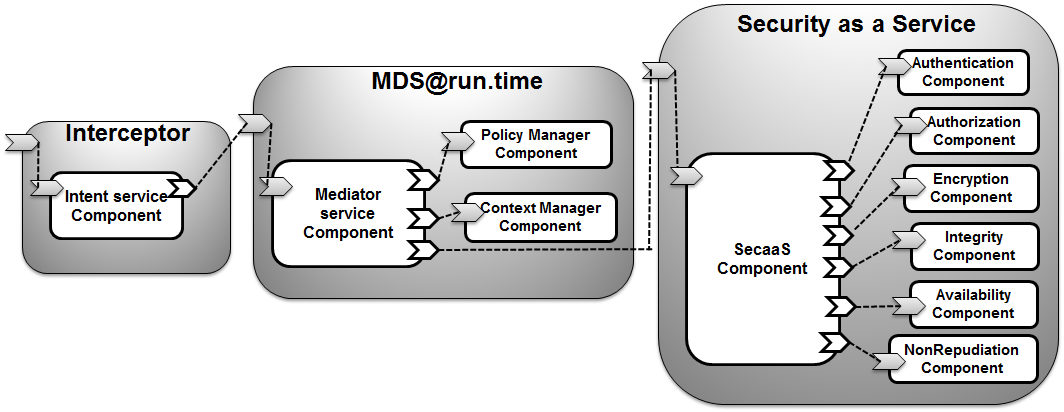
\includegraphics[height=150pt, width=350pt]{composites2.png}
\caption{MDS@run.time with FraSCAti.}
\label{fig:composites}
\end{figure}

\subsection{FraSCAti Intent for MDS@run.time}
SCA provides the notion of intent, which is an abstraction for designating a non-functional property such as security, transaction, logging, etc.
With FraSCAti, SCA intents are implemented as SCA components, then both business and non-functional concerns are designed then implemented in the same framework aka SCA.

The \texttt{Intent} component is responsible for detecting and intercepting business services invoked by clients. This component uses AOP techniques provided by FraSCAti to perform actions before, during and after each business service invocation. 
These techniques use the Apache CXF interception mechanism. The \texttt{Intent} component creates a \texttt{Request} object, which plays the intermediary role between the FraSCAti middleware and security services. This object provides a bidirectional interface that allows the \texttt{Intent} component to formalize the interaction messages received from Apache CXF and also to specify orders towards Apache CXF. The \texttt{Request} object ensures a total independence between our MDS@run.time components and the underlying service-oriented middleware, allowing on one hand the security services to be able to deploy and run on any other middleware and on another hand to deploy on a specific platform just the required security services.

\subsection{Composite MDS@run.time}
The \texttt{MDS@run.time} composite\footnote{An SCA composite is an SCA component containing a set of SCA components.} is invoked by the \texttt{Intent} component of the \texttt{Inter\-ceptor} composite. It includes:

\begin{itemize}
\settowidth{\leftmargin}{{\Large$\square$}}\advance\leftmargin\labelsep
\itemsep8pt\relax
\renewcommand\labelitemi{{\lower1.5pt\hbox{\Large$\square$}}}

\item The \texttt{Mediator} component is responsible for analyzing called service requests intercepted by the \texttt{Intent} component and  encapsulated into a \texttt{Request} object. It also identifies the security policy rules associated to business services invoked by clients. Thus, through the \texttt{Request} object, the \texttt{Mediator} receives information of the services involved in the interaction. This information is used to get policies associated to resources (the business services functionality implemented by the service operation). These policies are then analyzed and orchestrated by the \texttt{Mediator} to call the required security services.
\item The \texttt{PolicyManager} component manages the policies. It receives from the \texttt{Mediator} the resource or service reference requested and the link to the policy file. It returns to the \texttt{Mediator} the list of security policies to apply.
\item The \texttt{ContextManager} component analyses security policies associated to services and identifies the different policies to be applied according to the user context, the execution environment and security policies associated to the client and service provider. It also provides to the \texttt{Mediator} component information such as policies and policy rules related to the execution context. These policy rules are used by the \texttt{Mediator} component to call the technical security services.
\end{itemize}


\subsection{Composite SecaaS}

The \texttt{Security as a Service} composite is invoked by the \texttt{Mediator} component. It includes various security services, which allow protecting resources and business services according to a \textit{security as a service} approach. This composite contains the following components:


\begin{itemize}
\settowidth{\leftmargin}{{\Large$\square$}}\advance\leftmargin\labelsep
\itemsep8pt\relax
\renewcommand\labelitemi{{\lower1.5pt\hbox{\Large$\square$}}}

\item The \texttt{SecaaS} component is the composite entry point. It receives from the \texttt{Mediator} component the security policies to be applied. It is responsible for analyzing these policies, to identify the type of security services (authentication, authorization, etc.) to call.
\item The \texttt{Authentication} component is used to prove the user identity (of human or other service). This component receives from the \texttt{SecaaS} component the policy rule to apply, extracts information about the security pattern and invokes the security mechanism to be applied. It can be a weak authentication mechanism such as login/password or strong authentication such as One Time Password (OTP) or two factors authentication. This \texttt{Authentication} component includes subcomponents such as \texttt{SSORegistry} (Single Sign On Registry) component used to store information about  authentication of sessions and to allow to retrieve user information without restarting authentication.

\item The \texttt{Authorization} component allows managing access to resources and services, and allows grant or deny the user access to them. As the \texttt{Authentication} component, it receives the security policy rule and invokes the authorization mechanism to be applied. This mechanism can be based on an authorization by role (RBAC) implemented by the XACML authorization protocol or a simple Access Control List (ACL).
\item The \texttt{Encryption} component provides data and messages encryption/decryption mechanisms. It also provides secure protocols using secure communication (SSL).
\item The \texttt{Integrity} component ensures the integrity of exchanged data and messages by using message signatures or hash functions.
\item The \texttt{NonRepudiation} component is responsible for recording user actions (authentication, access to data or service, data modification/destruction, etc.). This information can then be used for auditing and monitoring.
\item The \texttt{Availability} component is responsible for the services' availability providing access to the service or a clone (redundant service) thereof if the original target service is unavailable. This component also provides backup mechanism to restore system data and services after disaster.

\end{itemize}

The \texttt{Encryption}, \texttt{Integrity} and \texttt{NonRepudiation} components can use security protocols such as WS-Security XML Encryption and XML Signature, which provide encryption and signing exchanged message mechanisms.


\section{Evaluation}

\label{sec:evaluation}


 Our performance evaluation is based on the use case presented in Section~\ref{example}, focusing on the \textit{ViewStudentData} operation. This operation is implemented thanks to a service associated to a security policy including authentication (see Fig.~\ref{fig:policy}, lines 2-8) by login/password (line 4) and access control (lines 9-16) using ACL (line 12) combined with a time constraint (line 10). As far as the e-government is concerned, the business service is encapsulated in an \textit{e-gov Scholarship service}, which is associated to the convenient security policy and refers to the \texttt{MDS@run.time} composite (Fig.~\ref{fig:gestionEtudiant}, line 6). By this way, the business service can be intercepted and MDS@run.time is invoked before invoking the business service itself.

\begin{figure}  
\center
\includegraphics[height=105pt,width=\linewidth]{scholarshipComposite.png}
\caption{Link the \emph{Scholarship} component with \textbf{MDS@run.time}.}
\label{fig:gestionEtudiant}
\end{figure}

% Fig.~\ref{fig:sequence} presents the runtime interactions of our different components. This figure has been produced by the FraSCAti Explorer tool~\cite{SMF09}, which captures component interactions as UML sequence diagrams.

% \begin{figure}  
% \center
% 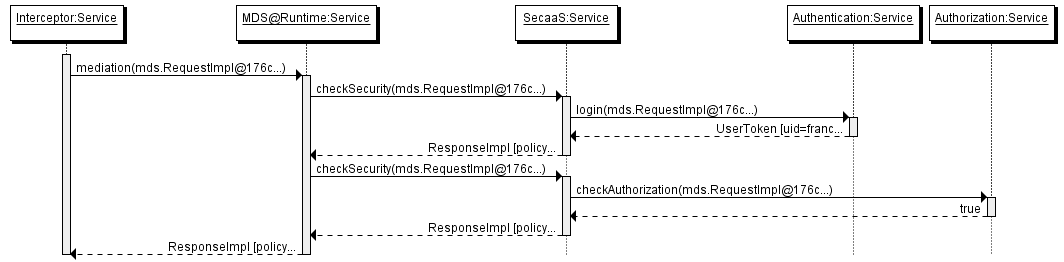
\includegraphics[height=120pt,width=\linewidth]{umlDiag.png}
% \caption{Interactions inside the \textbf{MDS@run.time} composite.}
% \label{fig:sequence}
% \end{figure}

To evaluate the impact of our \textit{MDS@run.time with FraSCAti} prototype on the service execution time, we set a test environment using FraSCAti version 1.6 with Oracle Java Virtual Machine 1.7.0\_51 on Microsoft Windows 7 Professional (32 bit) using a 2,54GHz processor Intel(R) Core(TM)2 Duo CPU with 4Go of memory.
We set different types of measures: A first execution invokes the business service without invoking our security architecture (measure 1 used to set a reference time), the time between the intent invocation and the MDS@run.time invocation measures the cost for the service interception. Then, the time required to get the policy file and parsed it is expressed by the mediation measure. Lastly execution times related to the authentication process and to the authorisation process are given.
We manage a test loop to compute an average time on 100 client requests, so that extra factor impacts can be smoothed, such as bootstrapping effects, Just-In-Time compilation, etc.

\begin{table}

\caption{Mean execution time of \textbf{MDS@run.time} components.}
%\begin{tabular}{|l@{}*{3}{|p{4.1cm}}|@{} }
\begin{tabular}{|p{0.4cm}|p{3.8cm}|c|c|}
\hline
No & Component &   Average execution  &  Average execution time / \\
 &  &   time (ms) &  Total execution time \\
  \hline
 1 & FraSCAti + Apache CXF + Business service & 59 &  76\%\\
2 & FraSCAti Interceptor & 2 &  3\%\\ 
3 & MDS@run.time & 4 &  5\%\\
 4 & Authentication& 10 & 13\%\\
5 & Authorization & 3 & 4\%\\
 \hline
 &  Total & 78 & 100\%\\
    \hline

\end{tabular}
\end{table}

The main result is that the interception and mediation process represents only 8\% of the total execution.
This overhead could certainly reduced within an industrial implementation of \textbf{MDS@run.time}.
However this demonstrates that our \textbf{MDS@run.time} approach, i.e. interpretation of security policies at runtime, introduces a small overhead compared to over protecting services.

\section{Related work}
\label{relatedwork}
Different strategies can be used to provide a consistent protection on distributed information systems, paying attention on both organisational and infrastructure related risks. 

On one hand, \textit{Security by Design} approaches integrate protection requirements while designing the information system. To this end, different frameworks have been defined to manage security annotations on UML diagrams (such as the multi-purpose UMLSec~\cite{JJ02} or the rather access control oriented  Secure UML~\cite{LBD02} domain specific languages) or BPMN diagrams (such as~\cite{WMS09} and~\cite{SSL09}). Taking advantage of such high-level specification, MDS~\cite{LS09}\cite{LZN14} adapts the Model Driven Engineering (MDE) approach to the security field. Several studies have focused on the use of the MDS approach to secure BP and led to frameworks definition like OpenPMF~\cite{LU10}, SECTET~\cite{AHB08} and BPSec~\cite{RFP07}. Nevertheless, none of them support the full transformation process. While BPSec is focused on the requirement engineering part (it includes CIM and PIM models), SECTET and Open PMF provide PIM, PSM and code generation features. Moreover, the generation process is achieved according to a static environment vision, i.e. they do not allow any adaptation depending on the execution context. This can lead to under or over protection depending on the real vulnerabilities/risks associated to the execution platform. Such static infrastructure vision also does not fit the scalable and elastic deployment provided by cloud environments.

On the other hand, \textit{Platform Dependent Protection} works have been conducted to organise a consistent protection level on cloud based infrastructure such as CSA protection stack~\cite{CSA11} whereas monitoring systems, such as intrusion Detection System~\cite{MPB12}, vulnerabilities checking~\cite{AVG11}, are used integrate information on the execution context and then the protection means accordingly. Nevertheless, these works are focused on a \textit{hosting platform protection} vision and do not integrate an end-to-end protection vision. To this end, the security stack defined in the OASIS Service reference model defines the way protection requirements should be implemented in a multi-layer architecture (application/Middleware-Transport/network) to improve the global protection consistency while deploying security features associated to a standardised security policy. Nevertheless, this coarse-grain model does not integrate any governance loop so that the execution context can be taken into account while deploying the required protection, leading to either over or under protection.
To overcome this limit, our MDS@run.time approach takes advantage of the OASIS security model and of the MDS approach to generate security policies depending on the collaborative BP organisational context~\cite{OFG13} so that services can be secured on demand. Moreover, it provides a fully oursourced security environment that can be plugged on any service-oriented middleware. Thanks to the execution platform information, collected by the \texttt{Mediator} component, security services are selected, composed and orchestrated in a transparent and consistent way, avoiding the costly over protection and the risky under protection.


\section{Conclusion}
Securing collaborative business process deployed on cloud systems requires paying attention on both organisational and platform-related vulnerabilities. Taking advantage of the intrinsic flexibility provided by the association of security policies to services, we propose to adapt and extend the MDS strategy to generate security policies and deploying them depending to the execution context. To this end, a MDS@run.time component is plugged on the middleware, paying attention on the hosting platform models to select, compose and orchestrate the security services depending on the required protection level and on the execution context.  The experiment reported in this paper shows how our MDS@run.time architecture can be plugged on the FraSCAti middleware and evaluate its performance level.
Further works will focus on the integration of more detailed platform models and on vulnerabilities monitoring loops so that our coarse-grained vision of the execution context will be refined to increase the protection efficiency.


% Utilisation de BibTex

 \bibliographystyle{splncs03}
 \bibliography{biblio} 

\end{document}

